\documentclass{article}
\usepackage{ctex}
\usepackage{amsmath}
\usepackage{amsthm}
\usepackage{amssymb}
\usepackage{anysize}
\usepackage{authblk} % 引入authblk包
\usepackage{graphicx}
\usepackage{media9}

\newtheorem{theorem}{定理}[section]
\newtheorem{proposition}[theorem]{命题}
\newtheorem{definition}[theorem]{定义}
\newtheorem{feature}[theorem]{性质}
\newtheorem{corollary}[theorem]{推论}
\newtheorem{example}[theorem]{例}
\newtheorem{lemma}[theorem]{引理}

\renewcommand{\i}{\mathrm{i}}
\renewcommand{\d}{\mathrm{d}}
\newcommand{\e}{\mathrm{e}}
\newcommand{\R}{\mathbb{R}}
\newcommand{\C}{\mathbb{C}}
\newcommand{\Z}{\mathbb{Z}}
\newcommand{\N}{\mathbb{N}}
\newcommand{\Q}{\mathbb{Q}}

\title{Stage 2 Problem 4}
\author{孙天阳\thanks{中国科学技术大学数学科学学院, \texttt{tysun@mail.ustc.edu.cn}}}
\date{\today}

\begin{document}
\maketitle
\begin{figure}[h]
    \centering
    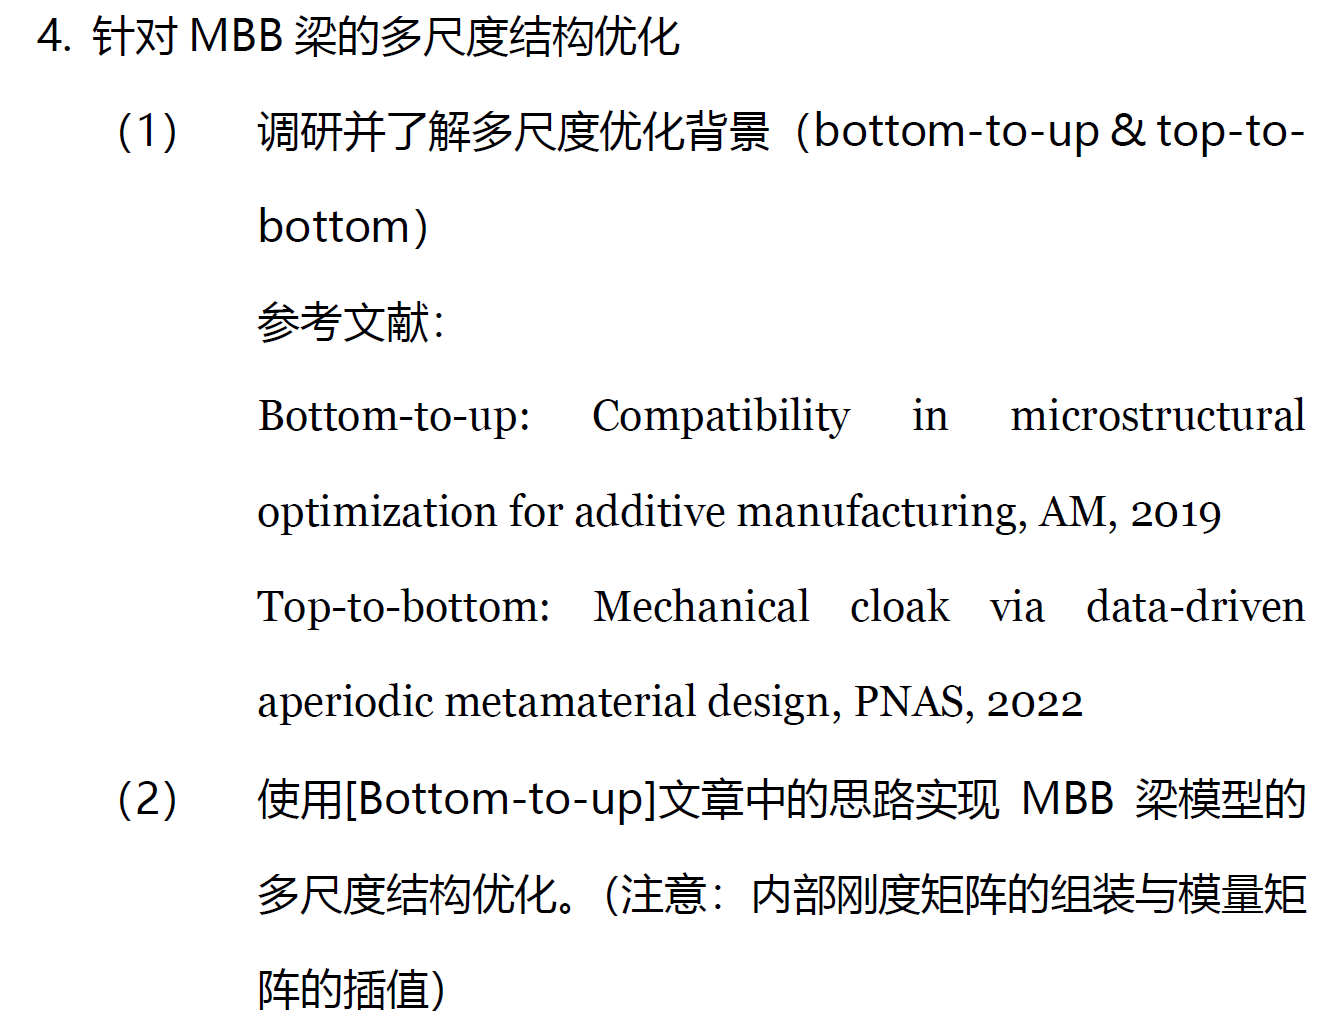
\includegraphics[width=0.8\textwidth]{Stage2_Problem4.png}
\end{figure}
\section{多尺度拓扑优化背景}
\begin{itemize}
\item 宏观拓扑优化:将设计区域如矩形划分单元格,每个单元格上的值在0到1之间变,灰度是不希望看到的,利用Heaviside投影得到黑白图,黑就是有材料,白就是没材料,设计出来的结果就像99行代码MBB梁的结果那样
\item 微结构拓扑优化:考虑一个单胞,这些单胞将被用来拼成宏观的弹性体,利用均匀化理论,我们可以通过优化单胞的结构来使得宏观的弹性体具有我们想要的性质,设计出来的结果就像夏凉2015年论文展示的结果那样
\item 多尺度拓扑优化:既进行宏观拓扑优化,每个单元格有一个0和1之间的值;又进行微结构拓扑优化,该单元格上的0到1之间的这个值就是这个单胞的体积分数,在满足这个体积分数的条件下这个单胞可以有自己的结构
\end{itemize}
实现多尺度拓扑优化有两类方法,多尺度的模型预先就假定了两个尺度;单尺度模型,只要划分足够细(不能施加消除网格依赖性的手段),也自然期待会出现微结构,之前的作业,Infill optimization for additive manufacturing—approaching bone-like porous structures,可以作为这个的例子。
\section{MBB梁的多尺度拓扑优化}






\end{document}